\documentclass{article}
\usepackage{pgf-umlcd}
\usepackage{tikz}

\begin{document}

\begin{center}
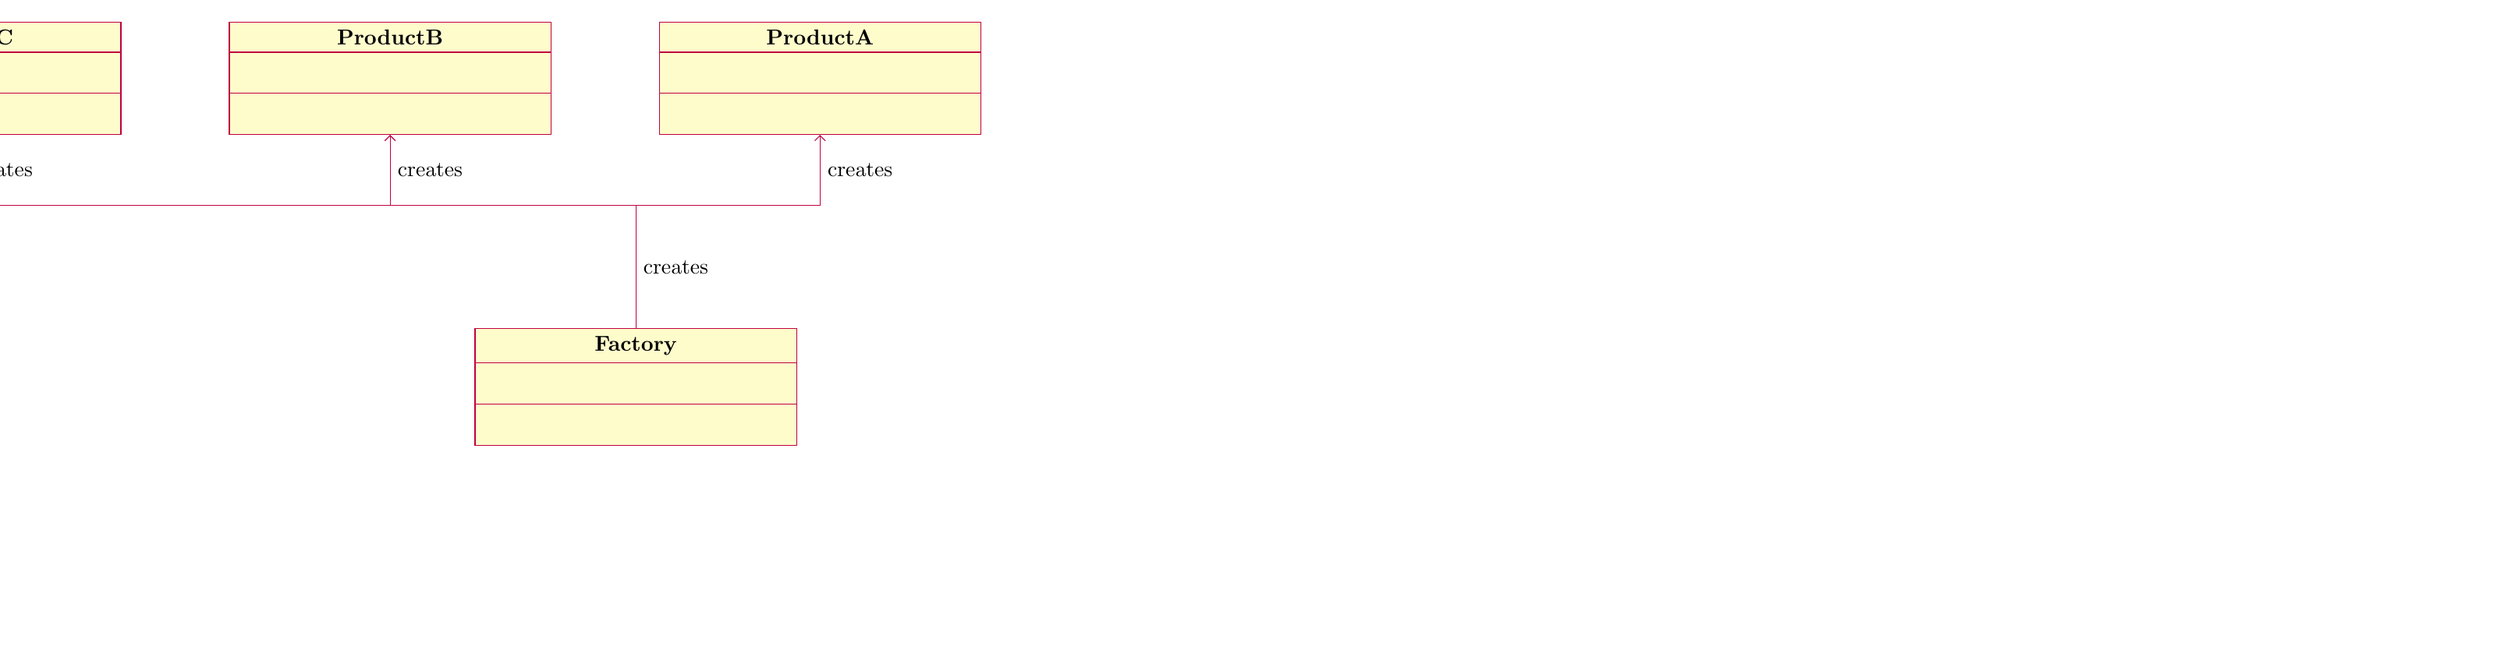
\begin{tikzpicture}
  \useasboundingbox (30,-5) rectangle (-10,5);
%   TODO: this is how to allow to place all over the place 

  % Factory Class at the center
  \begin{class}{Factory}{0,0}
    \attribute{}
    \attribute{}
    \operation{}
    \operation{}
  \end{class}

  % Product Classes, including ProductC
  \begin{class}{ProductA}{3,5}
    \attribute{}
    \attribute{}
    \operation{}
    \operation{}
  \end{class}

  \begin{class}{ProductB}{-4,5}
    \attribute{}
    \attribute{}
    \operation{}
    \operation{}
  \end{class}

  \begin{class}{ProductC}{-11,5} % Now it should work
    \attribute{}
    \attribute{}
    \operation{}
    \operation{}
  \end{class}

  % Connect Factory to Products
  \draw [umlcd style] (Factory.north) -- ++(0,2cm)
                      coordinate (tmp)
                      node[right,midway] {creates};

  \foreach \endpoint in {ProductA,ProductB,ProductC}
    \draw [umlcd style,fill=none,->] (tmp) -| (\endpoint.south)
                                     node[pos=0.75,right] {creates};

\end{tikzpicture}
\end{center}

\end{document}
